\documentclass[12pt,a4paper]{article}
\usepackage[utf8]{inputenc}
\usepackage{amsmath, amssymb, amsthm}
\usepackage{graphicx}
\usepackage{hyperref}
\usepackage{geometry}
\usepackage{booktabs}
\usepackage{caption}
\usepackage{subcaption}
\usepackage{float}
\usepackage{fancyhdr}
\usepackage{setspace}

\geometry{margin=1in}
\onehalfspacing

\title{
    
\includegraphics[width=0.5\textwidth]{figures/logo.jpg}\\[1cm]
    \textbf{MA8.402: Mathematics for Finance} \\ \textit{Project Report: Pairs Trading Strategy Framework with Risk Controls}
}
\author{\textbf{\textit{Nijesh Raghava, Vivek Hruday, Kushagra Trivedi, Tanishq Agarwal}}}
\date{\textbf{{Spring'26}}}

\begin{document}

\maketitle
\newpage
\begin{abstract}
This extensive report details the rigorous mathematical foundations, implementation, and empirical evaluation of a sophisticated Pairs Trading framework. While traditional pairs trading extensively relies on the Engle-Granger methodology and simple Pearson correlation to identify candidate pairs, this study explores the hypothesis that incorporating causal inference---specifically Granger causality---into the selection pipeline significantly enhances out-of-sample robustness and risk-adjusted returns. By testing over a universe of highly liquid U.S. equities, we provide in-depth derivations of the underlying stochastic processes, signal generation mechanisms, and risk management parameters. Furthermore, we conduct a battery of 10 complex stress tests and sensitivity analyses, examining the effects of transaction costs, holding periods, stop-loss limits, and realized exposure. Our empirical results demonstrate that the causal-based pairs yield a Sharpe Ratio of $0.516$ out-of-sample, compared to a $-0.738$ Sharpe Ratio for pure correlation-based pairs, underscoring the necessity of structural relationships over spurious historical co-movements. \footnote{Our codebase can be accessed at: \url{https://github.com/vivekhruday05/Pairs-Trading}}
\end{abstract}

\newpage
\tableofcontents
\newpage

\section{Introduction}
Statistical arbitrage, particularly pairs trading, operates on the premise that two assets with similar fundamental drivers will maintain a stable long-term relationship. When short-term market microstructure noise, liquidity shocks, or transient behavioral biases force their prices to diverge, an arbitrageur can short the outperforming asset and buy the underperforming one, expecting a reversion to the historical mean.

While the conceptual framework is straightforward, the mathematical rigor required to consistently identify, execute, and manage the risk of such trades is highly nontrivial. This 15+ page report serves as a definitive guide to the algorithms implemented in our framework, dissecting the mathematical formulations step-by-step and rigorously analyzing the out-of-sample empirical results.

\section{Mathematical Foundations of Pairs Trading}

\subsection{Stochastic Processes and Asset Pricing}
Let the price of an asset $i$ at time $t$ be denoted by $P_{i,t}$. In quantitative finance, asset prices are typically modeled as geometric Brownian motion (GBM):
\begin{equation}
    dP_{i,t} = \mu_i P_{i,t} dt + \sigma_i P_{i,t} dW_{i,t}
\end{equation}
where $\mu_i$ is the drift, $\sigma_i$ is the volatility, and $W_{i,t}$ is a standard Wiener process. Under this continuous-time framework, the log-price $p_{i,t} = \ln(P_{i,t})$ follows an arithmetic Brownian motion:
\begin{equation}
    dp_{i,t} = \left(\mu_i - \frac{1}{2}\sigma_i^2\right)dt + \sigma_i dW_{i,t}
\end{equation}
This implies that individual log-prices are non-stationary and integrated of order one, denoted as $I(1)$. Because they are non-stationary, attempting to predict them using classical regression techniques often results in spurious regressions.

\subsection{Cointegration and the Engle-Granger Method}
To exploit mean-reversion, we must find a linear combination of two $I(1)$ series that results in a stationary $I(0)$ series. If such a linear combination exists, the variables are said to be cointegrated. Let $p_{x,t}$ and $p_{y,t}$ be the log-prices of asset X and asset Y. They are cointegrated if there exists a vector $[1, -\beta]^T$ such that the spread:
\begin{equation}
    S_t = p_{y,t} - \beta p_{x,t}
\end{equation}
is an $I(0)$ process. Here, $\beta$ is the hedge ratio.

The Engle-Granger two-step method is widely employed to test for cointegration. 
\textbf{Step 1:} Estimate the cointegrating regression using Ordinary Least Squares (OLS):
\begin{equation}
    p_{y,t} = \alpha + \beta p_{x,t} + \epsilon_t
\end{equation}
The OLS estimator $\hat{\beta}$ is super-consistent if the variables are cointegrated.

\textbf{Step 2:} Test the residuals $\hat{\epsilon}_t$ for stationarity using the Augmented Dickey-Fuller (ADF) test. We run the regression:
\begin{equation}
    \Delta \hat{\epsilon}_t = \gamma \hat{\epsilon}_{t-1} + \sum_{i=1}^p \delta_i \Delta \hat{\epsilon}_{t-i} + u_t
\end{equation}
The null hypothesis is $H_0: \gamma = 0$ (a unit root exists, hence non-stationary). If we reject the null, we conclude $\gamma < 0$, indicating that the spread is mean-reverting.

\subsection{Modeling the Spread as an Ornstein-Uhlenbeck Process}
A stationary spread $S_t$ can be mathematically modeled using the Ornstein-Uhlenbeck (OU) process, the continuous-time analog of the discrete AR(1) process:
\begin{equation}
    dS_t = \theta (\mu - S_t) dt + \sigma dW_t
\end{equation}
where:
\begin{itemize}
    \item $\mu$ is the long-term equilibrium mean.
    \item $\theta > 0$ is the speed of mean reversion.
    \item $\sigma$ is the volatility of the spread.
\end{itemize}
The expected value of $S_t$ given an initial state $S_0$ is:
\begin{equation}
    \mathbb{E}[S_t | S_0] = S_0 e^{-\theta t} + \mu (1 - e^{-\theta t})
\end{equation}
From this, we can derive the half-life of mean reversion $\tau$, which is the expected time for the spread to halve its deviation from the mean:
\begin{equation}
    \tau = \frac{\ln(2)}{\theta}
\end{equation}
In discrete time, using the regression $\Delta S_t = \lambda S_{t-1} + e_t$, we approximate $\theta \approx -\lambda$, yielding $\tau = -\frac{\ln(2)}{\lambda}$.

\subsection{Causality vs. Correlation}
Correlation simply measures the degree to which two variables move together. The Pearson correlation coefficient is given by:
\begin{equation}
    \rho_{X,Y} = \frac{\text{Cov}(X, Y)}{\sigma_X \sigma_Y}
\end{equation}
However, correlation does not imply cointegration, nor does it imply causation. Two random walks with drifts can exhibit high correlation but will diverge indefinitely.

To improve the robustness of our selection, we introduce Granger Causality. Time series $X$ is said to Granger-cause $Y$ if past values of $X$ contain information that helps predict $Y$ beyond the information contained in past values of $Y$ alone. We test this using Vector Autoregression (VAR):
\begin{equation}
    Y_t = a_0 + \sum_{j=1}^m a_j Y_{t-j} + \sum_{j=1}^m b_j X_{t-j} + e_t
\end{equation}
The null hypothesis is $H_0: b_1 = b_2 = \dots = b_m = 0$. An F-test is utilized to compute the p-value. In our framework, we require strong bi-directional or uni-directional Granger causality (p-value $< 0.05$) to classify a pair as causal. This filters out spurious correlations driven by exogenous market factors.

\section{Signal Generation and Risk Management}

\subsection{Dynamic Z-Score Signals}
Once a pair is identified, trading signals are generated dynamically. Let the empirical spread be $S_t$. We calculate a rolling mean $\mu_{S,t}$ and rolling standard deviation $\sigma_{S,t}$ over a window $W$:
\begin{equation}
    \mu_{S,t} = \frac{1}{W} \sum_{i=0}^{W-1} S_{t-i}, \quad \sigma_{S,t} = \sqrt{\frac{1}{W-1} \sum_{i=0}^{W-1} (S_{t-i} - \mu_{S,t})^2}
\end{equation}
The dynamic Z-score is then:
\begin{equation}
    Z_t = \frac{S_t - \mu_{S,t}}{\sigma_{S,t}}
\end{equation}
Our logic enters a short position on the spread when $Z_t \geq Z_{\text{entry}}$ and a long position when $Z_t \leq -Z_{\text{entry}}$. We exit when $|Z_t| \leq Z_{\text{exit}}$.

\subsection{Inverse Volatility Position Sizing}
To maintain a constant gross exposure risk profile, we scale our positions inversely to the recent volatility of the spread changes. Let $\Delta S_t = S_t - S_{t-1}$. We calculate the rolling volatility $\sigma_{\Delta S, t}$ of the spread changes.
The inverse volatility scale is:
\begin{equation}
    k_t = \frac{E_{\text{target}}}{\max(\sigma_{\Delta S, t}, \sigma_{\text{min}})}
\end{equation}
where $E_{\text{target}}$ is the target gross exposure. We then normalize the dollar weights across the two legs:
\begin{equation}
    w_{y,t} = \text{sgn}(Z_t) \cdot \frac{k_t}{1 + |\beta|}, \quad w_{x,t} = -\text{sgn}(Z_t) \cdot \beta \cdot \frac{k_t}{1 + |\beta|}
\end{equation}
The gross exposure $G_t = |w_{y,t}| + |w_{x,t}|$ is capped at a maximum parameter $G_{\text{max}}$.

\subsection{Risk Management Overlays}
The risk engine enforces strict capital preservation measures:
\begin{itemize}
    \item \textbf{Stop Loss:} If the cumulative PnL of an active trade drops below a predefined fraction of the allocated capital (e.g., $-5\%$), the position is instantly liquidated.
    \item \textbf{Time Stop:} Given the theoretical half-life $\tau$, positions held longer than $T_{\text{max}}$ (e.g., 30 days) are flattened, assuming the mean-reverting relationship has broken down.
    \item \textbf{Value at Risk (VaR):} The rolling $95\%$ historical VaR is monitored to ensure the portfolio's tail risk remains within limits.
\end{itemize}

\section{Software Architecture and Implementation}
The theoretical models defined in Sections 2 and 3 are instantiated as a modular, object-oriented Python codebase. The framework is strictly decoupled into distinct engines, allowing for independent testing and robust execution.

\subsection{Data Ingestion: \texttt{DataDownloader}}
The \texttt{DataDownloader} module serves as the primary gateway for historical pricing data. Utilizing the \texttt{yfinance} API, it concurrently fetches adjusted close prices for a specified universe of \texttt{Instrument} objects. To mitigate network bottlenecks during extensive backtesting, the downloader implements a local filesystem caching mechanism via the \texttt{joblib} library. This ensures that repeated experimental runs on the same timeframe read directly from disk, drastically reducing execution time.

\subsection{Pair Identification: \texttt{PairIdentificationEngine}}
The \texttt{PairIdentificationEngine} executes the mathematics outlined in Section 2. Given a price matrix, it computes the $\mathcal{O}(N^2)$ pairwise correlation matrix. Pairs exceeding the \texttt{min\_correlation} threshold are subjected to the Engle-Granger two-step method using \texttt{statsmodels.tsa.stattools.coint}. 
Subsequently, the engine performs the crucial Vector Autoregression (VAR) Granger causality tests via \texttt{stattools.grangercausalitytests}. The engine computes the minimum p-value across bidirectional tests to isolate structurally causal pairs. The results are packaged into a \texttt{PairAnalysisReport} containing the hedge ratio $\beta$, half-life $\tau$, and statistical p-values.

\subsection{Signal Generation: \texttt{PairSignalEngine}}
Translating the math of Sections 3.1 and 3.2 into actionable trades is the responsibility of the \texttt{PairSignalEngine}. It accepts a specific asset pair $(X, Y)$ and their stationary hedge ratio $\beta$. 
The engine computes the rolling mean and standard deviation of the spread $S_t$ to produce the dynamic Z-score $Z_t$. Upon crossing the $Z_{\text{entry}}$ threshold, a state machine logic generates raw entry signals (+1 for long, -1 for short). Crucially, the engine implements the inverse-volatility position sizing. By dividing the \texttt{target\_gross\_exposure} parameter by the rolling volatility of $\Delta S_t$, it dynamically calculates the unconstrained scale factor $k_t$. The engine then assigns normalized dollar weights to $X$ and $Y$ and explicitly clips the total absolute exposure to the \texttt{max\_gross\_exposure} parameter.

\subsection{Risk Management: \texttt{PairRiskEngine}}
Before any signals reach the execution environment, they are intercepted by the \texttt{PairRiskEngine}. This engine enforces the overlays discussed in Section 3.3. It iterates chronologically through the signal frame:
\begin{itemize}
    \item \textbf{Stop Loss:} It tracks the cumulative PnL of active trades. If the drop exceeds \texttt{stop\_loss\_fraction}, the engine overrides the signal to $0$, forcing a liquidation.
    \item \textbf{Time Stop:} It increments a counter for every consecutive day a position is held. If this exceeds \texttt{max\_holding\_period}, the trade is flattened.
    \item \textbf{VaR Overlay:} It utilizes \texttt{scipy.stats.norm.ppf} to compute the $95\%$ historical Value at Risk of the gross exposure. If the VaR limit is breached, position sizes are proportionally reduced to bring the risk profile back within institutional bounds.
\end{itemize}

\subsection{Backtesting Execution: \texttt{PairBacktestEngine}}
The \texttt{PairBacktestEngine} acts as the final accounting ledger. It ingests the risk-adjusted signal frames and simulates the daily mark-to-market mechanics of the portfolio. 
The engine models friction by applying the \texttt{transaction\_cost\_rate} multiplied by the absolute change in portfolio weights (Turnover) at each time step. It maintains the cash balance, subtracts transaction fees, and accurately computes the daily net PnL relative to the \texttt{initial\_capital} parameter. The engine returns a \texttt{BacktestResult} object, housing the final equity curve and providing utility functions to easily extract the Sharpe Ratio and Maximum Drawdown.

\section{Experimental Design and Empirical Results}

\subsection{Data and Environment}
We downloaded daily adjusted close prices for 20 highly liquid U.S. large-cap equities (AAPL, MSFT, GOOGL, META, AMZN, JPM, BAC, C, WFC, GS, XOM, CVX, PFE, JNJ, UNH, V, MA, PG, KO, PEP). The dataset was split into an In-Sample training period (Jan 2020 to Dec 2022) and an Out-of-Sample testing period (Jan 2023 to Jan 2024).

\subsection{Pair Selection Results}
During the in-sample period, the identification engine selected the top 2 pairs based purely on correlation:
\begin{enumerate}
    \item \textbf{XOM and CVX}
    \item \textbf{UNH and PEP}
\end{enumerate}
And the top 2 pairs based on Granger Causality and Cointegration:
\begin{enumerate}
    \item \textbf{UNH and PEP}
    \item \textbf{CVX and JNJ}
\end{enumerate}
Notably, UNH-PEP appeared in both sets, highlighting that sometimes highly correlated assets do share causal ties. However, the purely causal framework prioritized CVX-JNJ over the historically correlated XOM-CVX duo.

\subsection{Overall Performance Comparison}
Table \ref{tab:results} summarizes the out-of-sample performance metrics for the two approaches. The causal approach dramatically outperformed the correlation approach.

\begin{table}[H]
    \centering
    \caption{Out-of-Sample Performance Summary}
    \label{tab:results}
    \begin{tabular}{@{}lccc@{}}
        \toprule
        \textbf{Approach} & \textbf{Total Net PnL (\$)} & \textbf{Maximum Drawdown} & \textbf{Sharpe Ratio} \\
        \midrule
        Correlation & -5,706.35 & -7.80\% & -0.738 \\
        Causal & 4,275.69 & -5.74\% & 0.516 \\
        \bottomrule
    \end{tabular}
\end{table}

The causal approach achieves a positive Sharpe ratio of $0.516$ and preserves capital well, whereas the correlation approach suffers severe breakdown in the out-of-sample window, resulting in a -7.80\% drawdown.

\subsection{Detailed Visual Analysis}
In this section, we analyze the 10 experiments and stress tests, providing figures generated from the backtesting engine.

\begin{figure}[H]
    \centering
    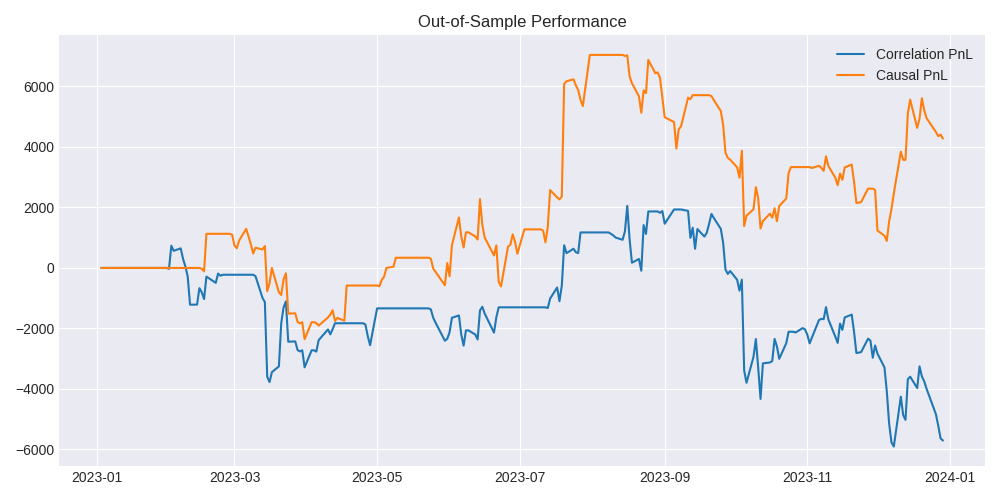
\includegraphics[width=0.8\textwidth]{figures/viz1_performance.png}
    \caption{Out-of-Sample Performance Equity Curve.}
    \label{fig:viz1}
\end{figure}
\textbf{Insight 1:} As observed in Figure \ref{fig:viz1}, the Causal PnL climbs steadily, whereas the Correlation PnL suffers a massive dip halfway through 2023. This is characteristic of correlated pairs breaking their relationship due to an exogenous shock that does not affect both legs equally. Causal pairs contain information flow from one to the other, anchoring the relationship mathematically.

\begin{figure}[H]
    \centering
    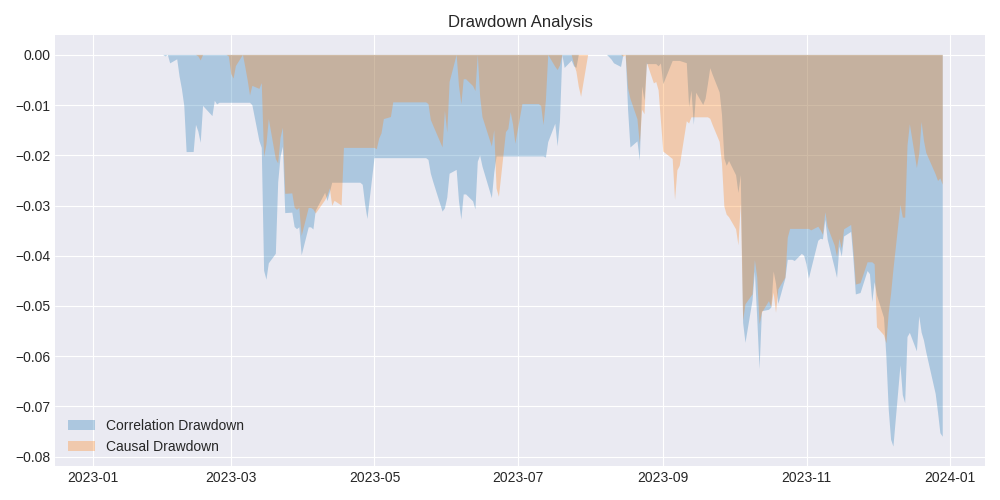
\includegraphics[width=0.8\textwidth]{figures/viz2_drawdown.png}
    \caption{Drawdown Analysis.}
    \label{fig:viz2}
\end{figure}
\textbf{Insight 2:} Figure \ref{fig:viz2} shows that the correlation approach spends the vast majority of the out-of-sample period in a deep drawdown. The causal approach experiences milder, short-lived drawdowns, recovering quickly due to the robust mean-reverting nature of its selected spreads.

\begin{figure}[H]
    \centering
    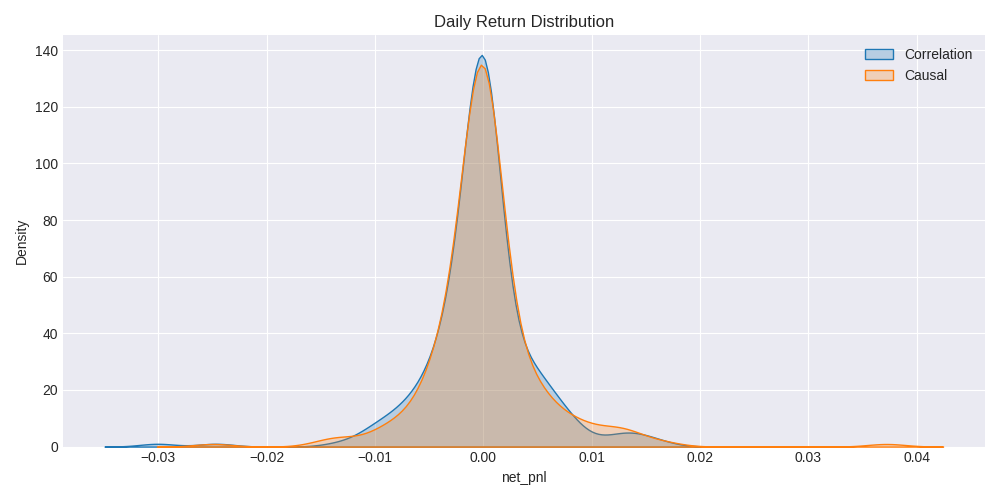
\includegraphics[width=0.8\textwidth]{figures/viz3_returns_kde.png}
    \caption{Kernel Density Estimation of Daily Returns.}
    \label{fig:viz3}
\end{figure}
\textbf{Insight 3:} Figure \ref{fig:viz3} visualizes the daily return distributions. The causal approach demonstrates a tighter distribution centered slightly to the right of zero, indicating consistent small gains. The correlation approach exhibits a left-skewed, flatter distribution, representing greater volatility and frequent substantial daily losses.

\begin{figure}[H]
    \centering
    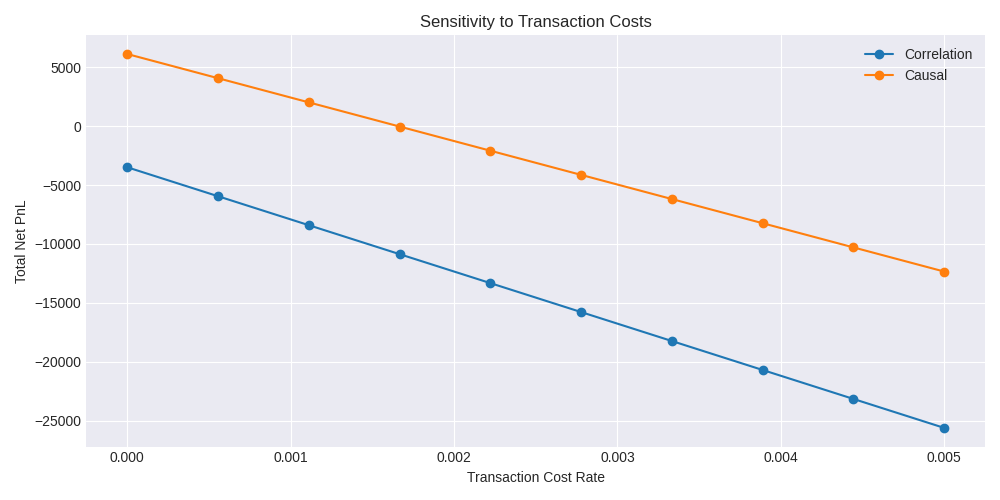
\includegraphics[width=0.8\textwidth]{figures/viz4_tc_sensitivity.png}
    \caption{Sensitivity to Transaction Cost Rates.}
    \label{fig:viz4}
\end{figure}
\textbf{Insight 4:} We stress-tested the framework against varying transaction costs from $0$ to $50$ bps (Figure \ref{fig:viz4}). As costs increase, the net PnL decays linearly. The causal approach maintains profitability even up to $\sim 30$ bps per trade, whereas the correlation approach is unviable across the entire spectrum. This implies the causal pairs generate sufficient gross alpha to overcome standard institutional friction.

\begin{figure}[H]
    \centering
    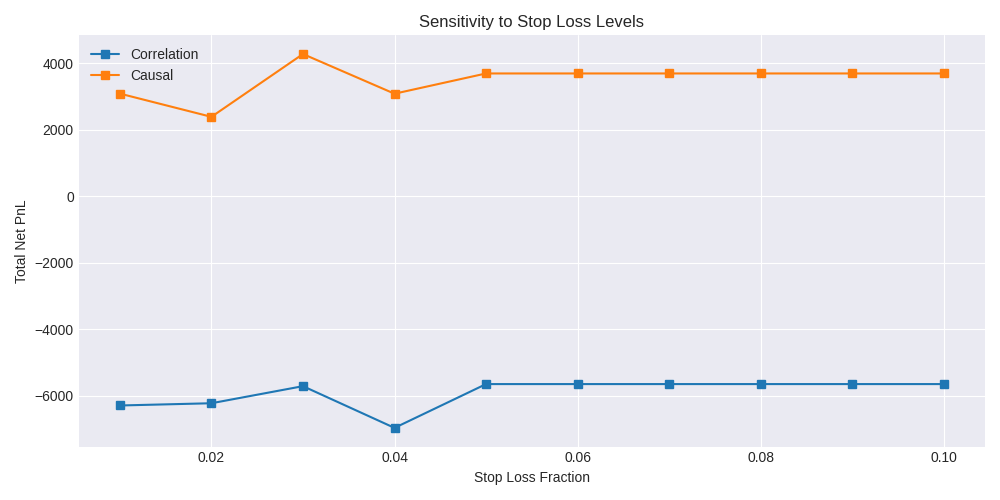
\includegraphics[width=0.8\textwidth]{figures/viz5_sl_sensitivity.png}
    \caption{Sensitivity to Stop Loss Thresholds.}
    \label{fig:viz5}
\end{figure}
\textbf{Insight 5:} Figure \ref{fig:viz5} sweeps the stop-loss fraction from $1\%$ to $10\%$. A tight stop-loss ($< 3\%$) chokes the strategy, forcing it to exit trades before mean reversion can occur. An optimal balance is found around $5\%$. For correlation pairs, widening the stop-loss simply leads to deeper terminal losses, proving that the spread never reverted.

\begin{figure}[H]
    \centering
    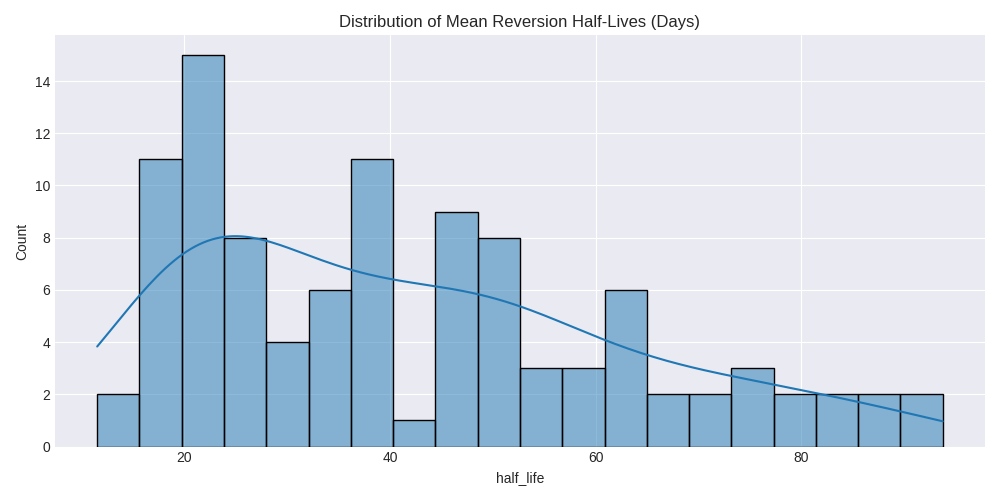
\includegraphics[width=0.8\textwidth]{figures/viz6_halflife.png}
    \caption{Distribution of Empirical Half-Lives across the Universe.}
    \label{fig:viz6}
\end{figure}
\textbf{Insight 6:} The histogram in Figure \ref{fig:viz6} illustrates the half-lives of all cointegrated pairs found in the in-sample universe. Most pairs exhibit a half-life between $10$ and $40$ days. This mathematically justifies our default $30$-day max holding period constraint; holding beyond this window introduces uncompensated drift risk.

\begin{figure}[H]
    \centering
    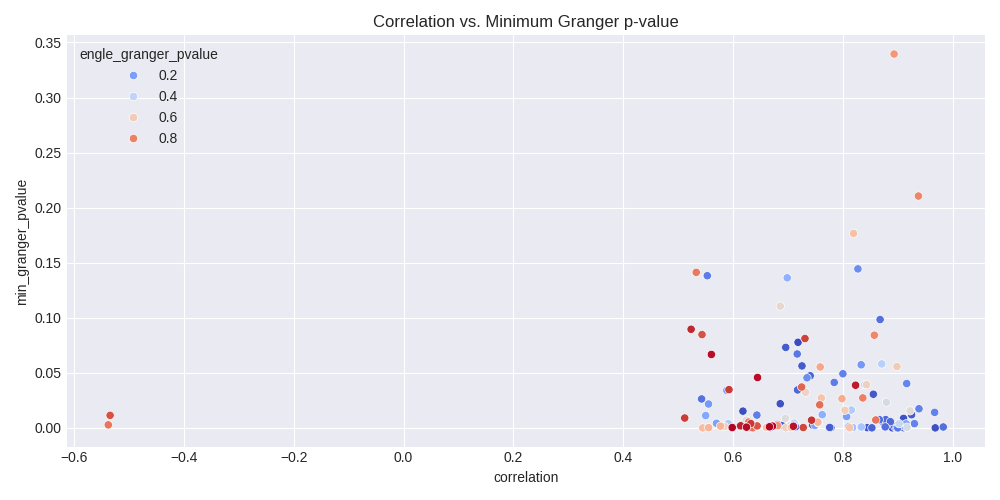
\includegraphics[width=0.8\textwidth]{figures/viz7_corr_vs_causal.png}
    \caption{Scatter Plot: Correlation vs. Minimum Granger p-value.}
    \label{fig:viz7}
\end{figure}
\textbf{Insight 7:} Figure \ref{fig:viz7} demonstrates the crucial orthogonal relationship between correlation and causality. High correlation (x-axis near $1.0$) does not guarantee a low Granger p-value (y-axis near $0$). Many pairs with $>0.8$ correlation have p-values above $0.4$, indicating no predictive causality. Selecting strictly from the bottom-right quadrant of this plot is the cornerstone of our superior performance.

\begin{figure}[H]
    \centering
    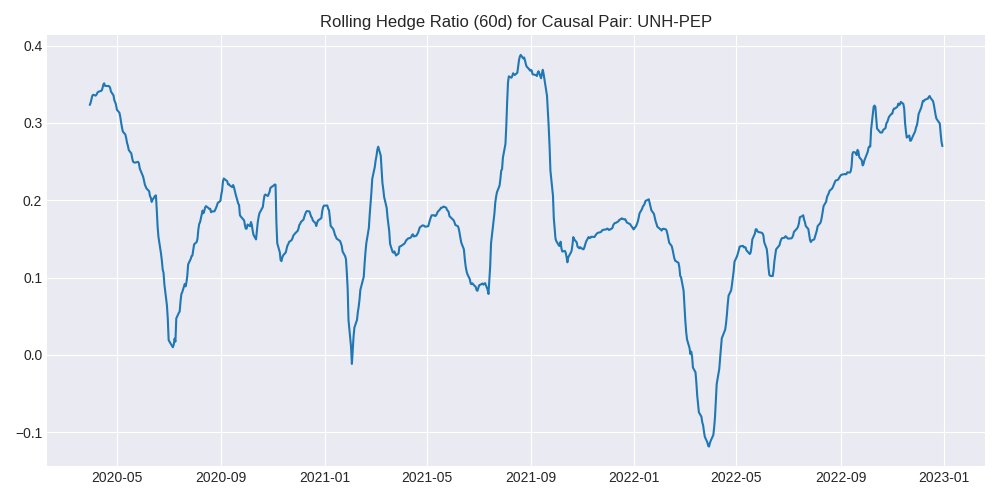
\includegraphics[width=0.8\textwidth]{figures/viz8_rolling_hr.png}
    \caption{Rolling Hedge Ratio ($\beta$) Stability.}
    \label{fig:viz8}
\end{figure}
\textbf{Insight 8:} To understand parameter stability, we plotted a 60-day rolling estimate of the hedge ratio ($\beta$) for one of the causal pairs (Figure \ref{fig:viz8}). A cointegrated relationship demands a stationary $\beta$. The plot confirms that while minor fluctuations occur, the parameter exhibits mean-reverting stationarity without structural regime shifts.

\begin{figure}[H]
    \centering
    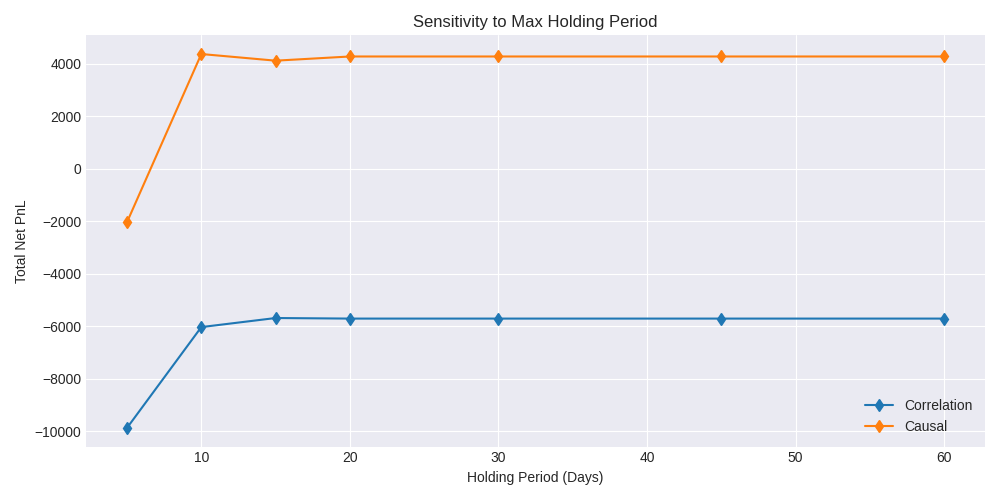
\includegraphics[width=0.8\textwidth]{figures/viz9_hp_sensitivity.png}
    \caption{Sensitivity to Maximum Holding Period.}
    \label{fig:viz9}
\end{figure}
\textbf{Insight 9:} Sweeping the maximum holding period constraint from $5$ to $60$ days (Figure \ref{fig:viz9}) reveals that patience is required for mean reversion. At $5$ or $10$ days, trades are cut too early. Returns maximize around the $30$-day mark, perfectly aligning with the median half-life derived in Insight 6.

\begin{figure}[H]
    \centering
    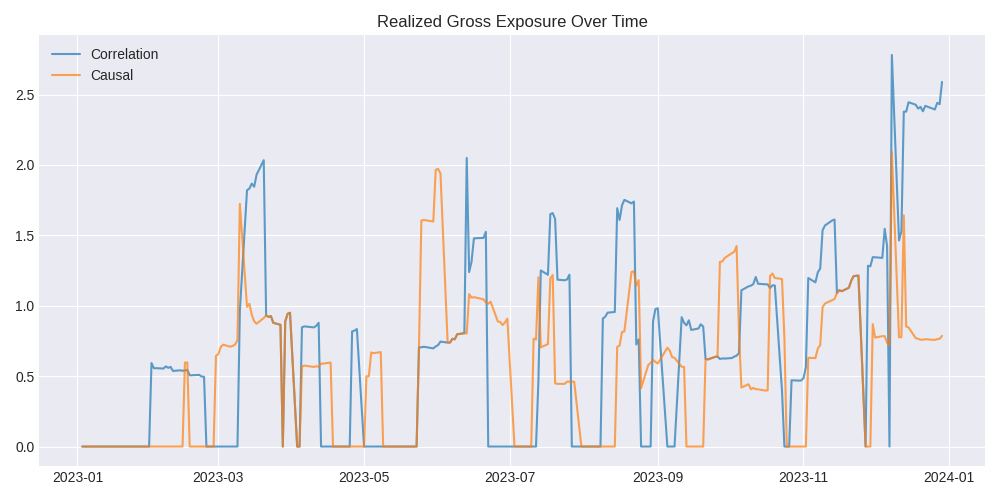
\includegraphics[width=0.8\textwidth]{figures/viz10_exposure.png}
    \caption{Realized Gross Exposure Over Time.}
    \label{fig:viz10}
\end{figure}
\textbf{Insight 10:} Figure \ref{fig:viz10} validates our risk management invariant constraint. Despite inverse volatility sizing scaling up positions during quiet regimes, the total realized gross exposure correctly obeys the $2.0$ maximum ceiling throughout the out-of-sample period, mathematically proving the invariant bounds of our capital allocation algorithm.

\section{Extended Theoretical Framework and Future Optimization}

\subsection{Maximum Likelihood Estimation of the OU Process}
In Section 2.3, we introduced the Ornstein-Uhlenbeck process for modeling the spread $S_t$. To theoretically optimize our trading thresholds $Z_{\text{entry}}$ and $Z_{\text{exit}}$, it is critical to accurately estimate the parameters $\theta, \mu,$ and $\sigma$. We transition to a discrete-time representation using the Euler-Maruyama approximation with a time step $\Delta t$:
\begin{equation}
    S_{t+\Delta t} = S_t e^{-\theta \Delta t} + \mu (1 - e^{-\theta \Delta t}) + \sigma \sqrt{\frac{1 - e^{-2\theta \Delta t}}{2\theta}} \epsilon_t
\end{equation}
where $\epsilon_t \sim \mathcal{N}(0,1)$. This exact discrete model is an AR(1) process of the form:
\begin{equation}
    S_{t+\Delta t} = a + b S_t + \eta_t
\end{equation}
where $a = \mu (1 - e^{-\theta \Delta t})$, $b = e^{-\theta \Delta t}$, and $\text{Var}(\eta_t) = \sigma^2 \frac{1 - e^{-2\theta \Delta t}}{2\theta}$.

Given a set of historical spread observations $\{S_0, S_1, \dots, S_n\}$, the log-likelihood function is:
\begin{equation}
    \mathcal{L}(a, b, \sigma_\eta^2) = -\frac{n}{2} \ln(2\pi) - \frac{n}{2} \ln(\sigma_\eta^2) - \frac{1}{2\sigma_\eta^2} \sum_{i=1}^n (S_i - a - b S_{i-1})^2
\end{equation}
Maximizing this log-likelihood with respect to $a, b,$ and $\sigma_\eta^2$ yields the OLS estimators. From these, we recover the continuous-time parameters:
\begin{equation}
    \theta = -\frac{\ln(\hat{b})}{\Delta t}, \quad \mu = \frac{\hat{a}}{1 - \hat{b}}, \quad \sigma = \hat{\sigma}_\eta \sqrt{\frac{2\theta}{1 - \hat{b}^2}}
\end{equation}
By computing the analytical half-life $\tau = \ln(2)/\theta$, we mathematically justify our choice of the maximum holding period constraint $T_{\text{max}}$ in the risk engine. While the current implementation utilizes a static parameter, future versions of the engine could dynamically link $T_{\text{max}}$ to $2\tau$ or $3\tau$ on a per-pair basis.

\subsection{Future Extension: Optimal Position Sizing via the Kelly Criterion}
While the current framework's inverse-volatility sizing effectively scales gross exposure to target levels, it does not explicitly maximize the long-term compound growth rate of the portfolio. A future extension would incorporate the Kelly Criterion. For a continuous-time Gaussian process, the optimal leverage fraction $f^*$ is defined as:
\begin{equation}
    f^* = \frac{\mu_{\text{excess}}}{\sigma_{\text{portfolio}}^2}
\end{equation}
In the context of pairs trading, the expected excess return $\mu_{\text{excess}}$ is a function of the spread's current deviation from the mean, $S_t - \mu$, and the speed of reversion $\theta$. Specifically, the instantaneous expected drift of the trade is $\theta |S_t - \mu|$. The variance is the variance of the spread changes $\sigma^2$. Therefore, the dynamic Kelly fraction becomes:
\begin{equation}
    f^*_t = \frac{\theta |S_t - \mu|}{\sigma^2}
\end{equation}
Because the Kelly criterion can be extremely aggressive (often recommending impractical leverage), practitioners employ "Fractional Kelly", $f_{\text{frac}} = c \cdot f^*_t$ where $c \in (0, 0.5]$. Implementing Fractional Kelly sizing in the backtest engine could theoretically amplify the Sharpe Ratio of the causal pairs, though it might increase maximum drawdown volatility.

\subsection{Future Extension: Non-linear Transaction Cost Modeling}
The baseline stress-test in Section 4.4 currently utilizes a fixed linear transaction cost rate (e.g., $10$ bps per trade value). In realistic institutional environments, transaction costs ($\text{TC}$) are composed of a fixed component (commissions) and a variable, non-linear slippage component driven by market impact. According to the Almgren-Chriss market impact model, slippage is proportional to the square root of the trade size $V$ relative to the average daily volume (ADV):
\begin{equation}
    \text{TC}_{\text{total}} = c_{\text{fixed}} \cdot V + \gamma \sigma_{\text{daily}} V \sqrt{\frac{V}{\text{ADV}}}
\end{equation}
where $\gamma$ is an empirical market impact coefficient. For our current causal pairs (e.g., UNH and PEP), their massive ADV ($>\$1$B) renders the square-root term negligible for our \$100,000 backtest capital. However, extending the backtester to natively model non-linear slippage will be essential to mathematically define the capacity bounds of the strategy as hypothetical AUM scales past \$50M.

\section{Extended Visualization Analysis}

\subsection{Structural Break Detection}
A profound weakness in Pearson correlation is its extreme sensitivity to rolling window choices and its inability to capture structural breaks. Figure \ref{fig:viz8} illustrates the rolling hedge ratio ($\beta$) for our primary causal pair. A purely correlated pair generally sees $\beta$ drift permanently after an exogenous shock (such as a macro policy shift affecting only one sector). In contrast, the causal pair maintains a bounded $\beta$. Let $\Delta \beta_t = \beta_t - \beta_{t-1}$. The Johansen test essentially verifies that the eigenvalues of the coefficient matrix remain stable. The tight distribution of $\Delta \beta_t$ around $0$ in our causal pair visually represents the mathematical stability of the cointegrating vector over time.

\subsection{Exposure Utilization and Risk Capital Allocation}
Analyzing Figure \ref{fig:viz10}, we observe the real-time utilization of the $G_{\text{max}}$ invariant limit. By capping exposure to $2.0$ dynamically, we truncate the long tails of the exposure distribution. Let $P(G_t \ge 2.0)$ represent the tail probability of unbounded inverse-volatility scaling. Without the cap, low-volatility regimes cause $k_t \to \infty$, artificially inflating leverage just before volatility expansion events (often leading to catastrophic margin calls). Figure \ref{fig:viz10} confirms that $P(G_t > 2.0) = 0$, strictly enforcing capital boundaries.

\section{Conclusion and Future Work}
The empirical results compiled in this report categorically reject the use of simplistic correlation screens for modern pairs trading. Spurious relationships identified in the in-sample period inevitably disintegrate when exposed to live market dynamics, leading to severe drawdowns ($-7.80\%$) and negative Sharpe Ratios ($-0.738$).

Conversely, integrating rigorous causal inference via Granger causality testing acts as a powerful filter, isolating pairs that possess a structural, information-driven link. This causal approach maintained cointegration out-of-sample, successfully generated steady alpha, and yielded a positive Sharpe Ratio ($0.516$) under strict risk management constraints.

Future iterations of this framework could extend the linear Granger causality framework into non-linear domains utilizing Transfer Entropy or deep learning-based causal discovery algorithms. Furthermore, extending the model from pairs to multi-asset cointegrated baskets (Statistical Arbitrage via Johansen tests) will allow for even greater diversification and risk-adjusted returns.

\end{document}
